%\documentclass[a4paper]{report}
\documentclass[a4paper,11pt]{report}
\usepackage[utf8]{inputenc}
\usepackage[portuguese]{babel}
%\usepackage[portuges]{babel}
\usepackage{graphicx}
\usepackage{hyperref}
\usepackage{float}

\usepackage{geometry}
 \geometry{
 a4paper,
 total={170mm,257mm},
 left=25mm,
 right=25mm,
 top=20mm,
 }

\graphicspath{ {./images/} }

\begin{document}


\title{Relatório Trabalho Prático LI3 em C}
\author{Grupo 58\\
\\
João Azevedo, Paulo Araújo e Pedro Machado}
\date{\today}

\begin{figure}[t]
  \centering
  
\includegraphics[scale=0.5]{uminho.png}
  \label{img:logo}
\end{figure}

\maketitle

%\tableofcontents

%\listoffigures

%\listoftables

%% Introdução
\chapter{Introdução}

\quad A Unidade Curricular (UC)  Laboratórios de Informática III é uma unidade curricular do curso de Mestrado Integrado em Engenharia Informática (MiEI). Esta UC tinha como objetivo a consolidação experimental dos conhecimentos teóricos e práticos adquiridos nas UCs anteriores e na introdução de novas técnicas de programação fundamentais na área de desenvolvimento de software com grandes quantidades de dados e com mais elevada complexidade algorítmica e estrutural.


\section{Objectivos}

\quad O projeto tinha como objetivo simular um Sistema de Gestão Vendas (SGV) de vários SuperMercados da mesma marca, mais concretamente três. Nesta aplicação o utilizador consegue aceder às informações das vendas, cujas possuem informação relativa às 3 filiais da marca, produtos comprados, clientes que efetuaram as compras, o mês em que a compra foi realizada, se o produto se encontrava em promoção, o preço do produto,…
Para além das vendas efetuadas, a aplicação contém os Produtos totais disponíveis, bem como os clientes.
A principal preocupação da aplicação tende com o desempenho a nível de tempo depois de receber um 'input' por parte do utilizador. Desta preocupação resultaram várias tentativas e medições de tempo em relação à estrutura de dados, bem como a modularidade, até o código final.


\chapter{Estruturas de Dados e Módulos (API.h)}
\quad Em termos gerais, todos os nossos módulos principais (Filial, Faturação e os catálogos de Produtos/Clientes/Vendas) dependem de uma estrutura principal usada para um armazenamento ordenado dos dados.

\quad Esta estrutura de dados é uma simples AVL (balanced binary tree) que dispõem, no módulo "avlstruct.h", de operações elementares de inserção (update), de inicialização (initAVL) e de rotações à direita/esquerda bem como as funções responsáveis por tratar do balanceamento da mesma.


\section{Catálogos de Produtos, Clientes e Vendas:}

\quad Nos catálogos de produtos e clientes, a AVL apresenta-se ordenada por um elemento lá denominado por "tag" que representa o produto (ou cliente) que pertence à AVL, como se vê na Figura \ref{fig1}. No módulo vendas, a sua AVL apresenta-se ordenada da mesma forma apresentando ainda um campo REGISTO que guarda os campos da string venda lida do ficheiro (e validada), como se vê na Figura \ref{fig2}.

\begin{figure}[h!]
  \centering
  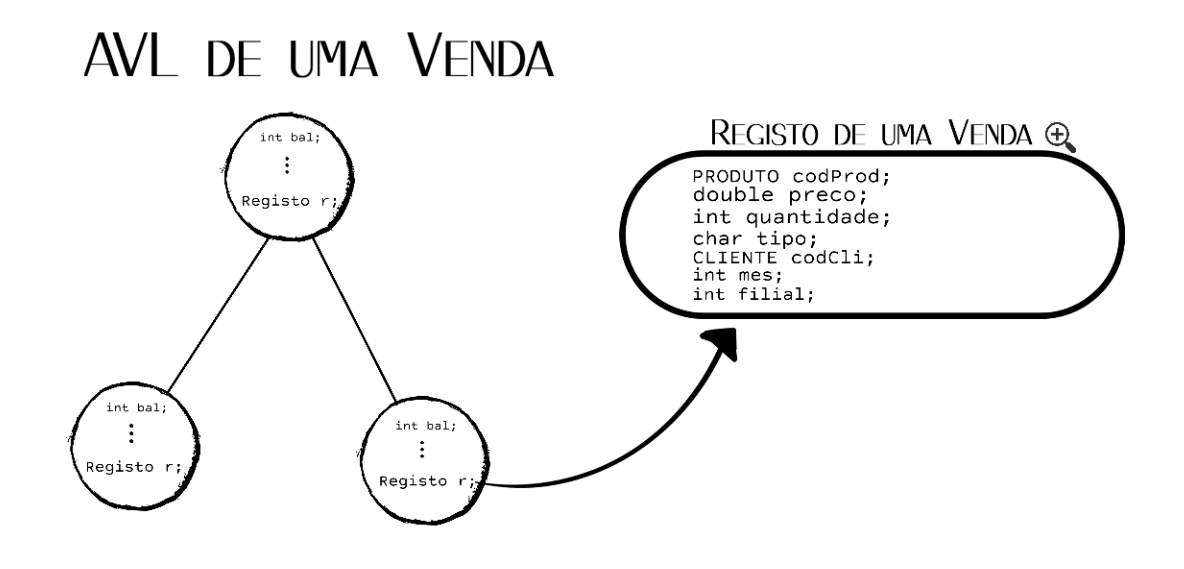
\includegraphics[scale=0.20]{Avl_Venda.png}
  \caption{Imagem da Estrutura da AVL Vendas.}
  \label{fig1}
\end{figure}

\begin{figure}[H]
  \centering
  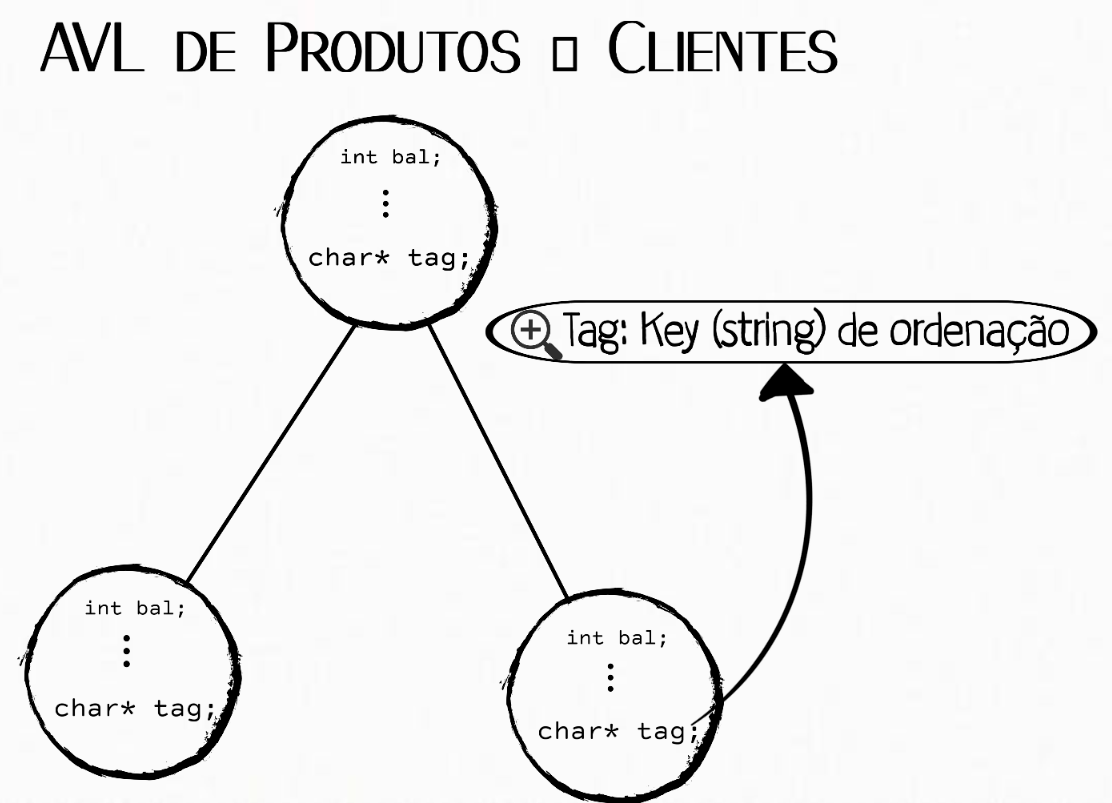
\includegraphics[scale=0.15]{Avl_Prod_Cli.png}
  \caption{Imagem da Estrutura da AVL Clientes e Produtos.}
  \label{fig2}
\end{figure}


%TENTAR METER O TEXTO DEPOIS DA IMAGEM 

Ora, esta organização permite-nos uma ordenação catalogada por ordem alfabética permitindo tirar partido, como pretendido, da AVL. Para além disso, temos a nuance de possuir todos os campos da struct AVL passando a NULL os que não são utilizados, como por exemplo: Para o catálogo de produtos interessa ter o campo "tag" diferente de NULL (ou seja, com o Produto lá armazenado) mas todos os outros campos da struct são enviados nas funções de update a NULL (não utilizando, assim, memória desnecessariamente).

\section{Módulo Faturação}
\quad Este módulo contém estruturas de armazenamento de toda a faturação gerada por um dado produto da AVL vendas: Trata-se de um array de AVL's de faturação com 3 posições, correspondendo a cada uma a filial respetiva. Cada nodo da AVL de faturação possui uma estrutura extra ("FATURA f" p. exe.) que armazena um produto e duas matrizes contendo a Faturação e número de vendas desse produto dividida pelos 12 meses e pelos dois tipos de venda (N e P), como se vê na Figura \ref{fig3}.

%METER A IMAGEM DEPOIS DE FATURAÇÃO
\begin{figure}[h!]
  \centering
  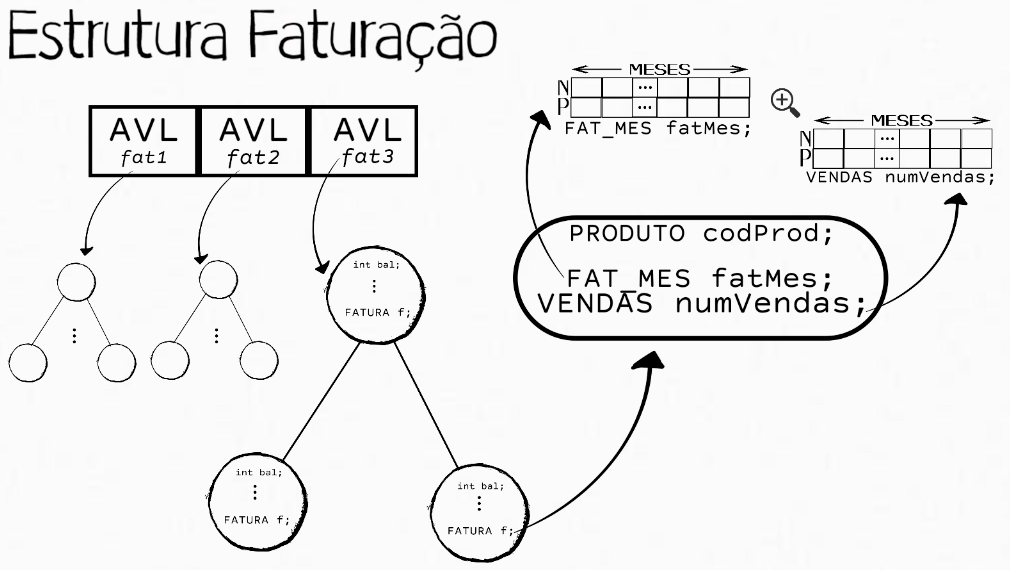
\includegraphics[scale=0.20]{Faturacao.png}
  \caption{Imagem da Estrutura da Faturação.}
  \label{fig3}
\end{figure}

A escolha detalha destes critérios, permite-nos aumentar a filtragem dos resultados para as queries de modo a tornar mais eficiente as operações de procura. A divisão em arrays permite-nos a filtragem da filial que aliado à organização da AVL por ordem alfabética do produto é uma das principais vantagens e, para além disso, a organização das matrizes por mês e tipo poupam o trabalho de fazer procuras extras desnecessárias. Em termos de exemplos concretos, a query 3 tira bastante partido dessa organização visto que filtra as compras num mês para um dado produto.


\section{Módulo Filial}
Este módulo, pelo contrário, já conhece clientes e as suas compras/produtos adquiridos em cada filial. Encontra-se, da mesma forma, dividido num array de filiais, na qual cada posição possui uma AVL filial que contém o código do cliente e uma lista de produtos adquiridos onde, em cada produtos temos associado a faturação do mesmo e a quantidade adquirida, mês a mês entre os tipos N e P, como se vê na Figura \ref{fig4}

%METER A IMAGEM DEPOIS DE FILIAL
\begin{figure}[h!]
  \centering
  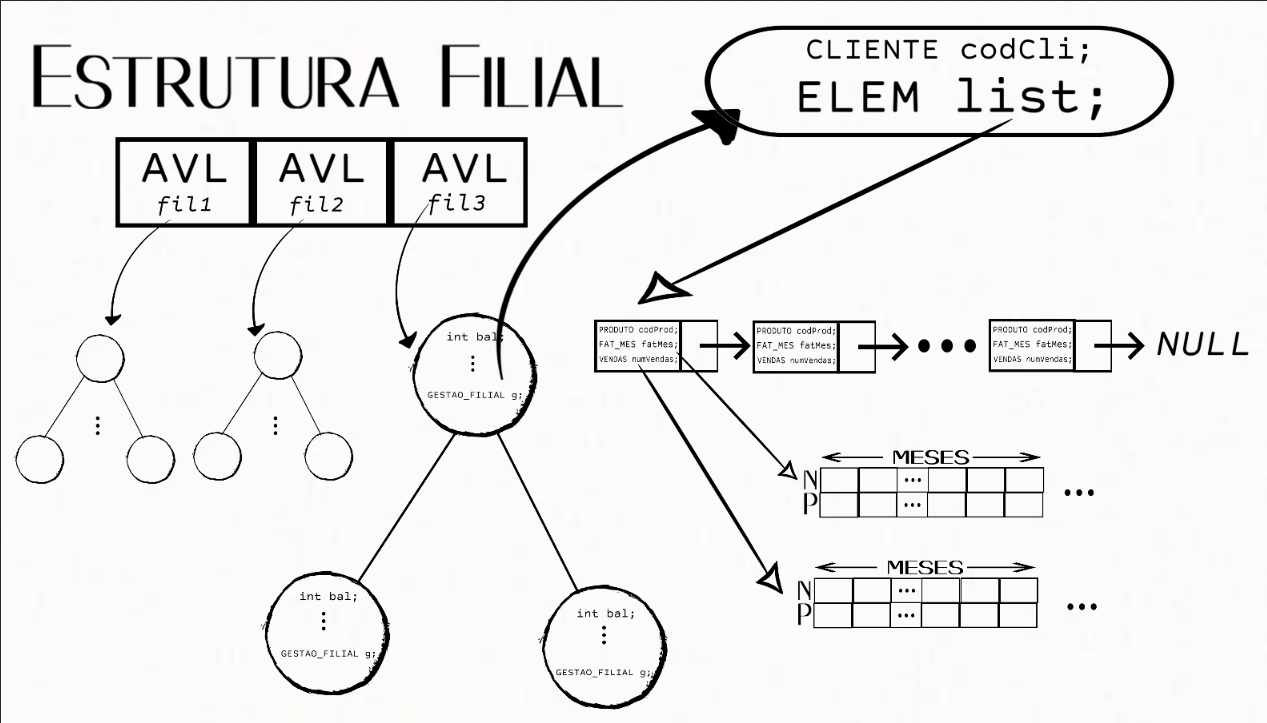
\includegraphics[scale=0.20]{Filial.png}
  \caption{Imagem da Estrutura da Filial.}
  \label{fig4}
\end{figure}

Como esta estrutura, ou melhor, parte dela se assemelha à descrita anteriormente, também apresenta eficiência na procura dos dados. Indo a exemplos concretos, as query 6 e 7 que não implicam um varrimento total das estruturas e tiram proveito da organização das matrizes para verificar numa as que se encontram a zeros (indicação de produto não adquirido) e por outro lado a criação das tabelas de compras realizadas por um dado cliente numa filial.

\section{Outras Estruturas}

\subsection{Hashtables}
\quad Também foi importante a utilização de hashtables em termos de organização de dados para a resolução da query 11, em particular, de modo a tirar proveito das funções de lookup (com complexidade O(1)), isto é, associadas também a uma boa função de hash.

A nossa função de hash, após diversos testes de colisões, utiliza os números presentes na String Produto (4 números) para gerar o hashcode para um determinado produto com um número elevadíssimo de combinações. Aliado a isso utilizamos quadratic probing visto que se revelou mais rápido na criação da hashtable.

\subsection{Linked list}
\quad Após vários testes verificámos que um cliente não compra, em geral, mais de 10 produtos, para isso, utilizamos estruturas ligadas de apontadores para armazenar informação que nunca excede grandes dimensões, nomeadamente na estrutura filial ao armazenarmos a lista de produtos comprados por um cliente.



\chapter{Interface com o Utilizador}
\quad A Interface do Utilizador com o Sistema de Gestão Vendas (SGV) é garantida através de um conjunto de queries, mas especificamente 12. Estas 12 queries servem para o utilizador ter uma noção dos dados que o SGV gere.


\section{Queries}
\label{sec:Queries}

\subsection*{Query 1}
\label{sec:Query1}

Na query um, era pretendido apresentarmos as informações em relação aos dados recebidos das vendas, produtos e clientes.

\subsection*{Query 2}
\label{sec:Query2}

Na segunda query, era pedido para indicarmos uma lista dos produtos que começassem pela letra indicada pelo utilizador. Para além disto, deveríamos apresentar essa lista organizada por páginas que possibilitassem a sua navegação.


\subsection*{Query 3}
\label{sec:Query3}

A terceira query pedia para dado um mês e um código de produto, ambos válidos, determinar e apresentar o número total de vendas e o total faturado com esse produto em tal mês, distinguindo os totais em modo N e os totais em modo P, ou seja, destinguir aqueles produtos que estavam em promoção (P) e os que não estavam (N).
O utilizador poderá decidir se pretende o resultado global ou os resultados filial a filial para todas as 3 filiais.

\subsection*{Query 4}
\label{sec:Query4}

A query quatro pretendia determinar a lista ordenada dos códigos dos produtos (e o seu número total) que ninguém comprou, podendo o utilizador decidir se pretendia valores totais ou divididos pelas filiais.

\subsection*{Query 5}
\label{sec:Query5}

Na query cinco era pretendido determinar a lista ordenada de códigos de clientes que realizaram compras em todas as filiais.

\subsection*{Query 6}
\label{sec:Query6}

A query seis pedia para determinar o número de clientes registados que não realizaram compras bem como o número de produtos que ninguém comprou.

\subsection*{Query 7}
\label{sec:Query7}

Na sétima query, era pretendido que dado um código de cliente, criar uma tabela com o número total de produtos comprados (ou seja a soma das quantidades de todas as vendas do produto), mês a mês e organizada por filial.

\subsection*{Query 8}
\label{sec:Query8}

A query oito, pedia que dado um intervalo fechado de meses, por exemplo [1..3], determinássemos o total de vendas registadas nesse intervalo e o total faturado.

\subsection*{Query 9}
\label{sec:Query9}

Na query nove, era pretendido que dado um código de produto e uma filial, determinássemos os códigos (e número total) dos clientes que o compraram, distinguindo entre compra N e compra P.

\subsection*{Query 10}
\label{sec:Query10}

A query dez, pedia que dado um código de cliente e um mês, determinássemos a lista de códigos de produtos que mais comprou por quantidade, por ordem descendente.

\subsection*{Query 11}
\label{sec:Query11}

Na query onze, era pedido para criar uma lista dos N produtos mais vendidos em todo o ano, indicando o número total de clientes e o número de unidades vendidas, filial a filial.

\subsection*{Query 12}
\label{sec:Query12}

Na décima segunda query era pretendido que dado um código de cliente, determinássemos quais os códigos dos 3 produtos em que mais gastou dinheiro durante o ano.

\chapter{A Nossa Solução}
\label{sec:solucao}
\quad Como ainda estamos a iniciar a nossa aprendizagem na área de programação foi-nos proposto a execução do projeto pela realização de seis tarefas.
Desta forma, fomos capazes de abordar os problemas por etapas, focando-nos numa tarefa de cada vez.

\section*{Query 1}
A nossa resolução da query foi validar os ficheiros de produtos, clientes e vendas conforme os requisitos do SGV. Aqui damos a conhecer ao utilizador quantas vendas, produtos e clientes foram validados, o número de caracteres da linha mais longa,…

%\bigskip
\section*{Query 2}
Para esta query decidimos criar uma estrutura simples, semelhante a uma Stack, com vista a guardar os produtos pretendidos.


%\bigskip
\section*{Query 3}
Nesta querycriamos duas matrizes, a partir do produto e mês fornecido pelo utilizador, com o objetivo de guardar o número total de vendas numa e noutra o total faturado. As matrizes foram desenhadas para distinguir as 3 filiais e ainda os modos (N e P).


%\bigskip
\section*{Query 4}
Nesta query decidimos que os valores totais se referem aos produtos que não foram comprados nas três filiais. Já os resultados filial a filial, que se referiam aos produtos que não foram comprados na filial 1, e o mesmo para a 2 e 3, apresentando a lista para cada filial individualmente.

%\bigskip
\section*{Query 5}
Nesta query percorremos a estrutura Filial e caso o cliente exista nas 3 filiais adicionamos à lista, neste caso uma AVL, sendo que esta fica ordenada.

%\bigskip
\section*{Query 6}
Na query seis percorremos a estrutura Filial através da AVL clientes para calcular o número de clientes que não efetuaram compras, ou seja, que não se encontravam na estrutura Filial.
Efetuamos o mesmo raciocínio para os produtos, mas desta vez percorremos a estrutura Faturação através da AVL produtos.

%\bigskip
\section*{Query 7}
Para esta query criamos uma matriz para representar a tabela pretendida. Assim, percorremos a estrutura Filial e fomos somando, caso fosse o cliente pretendido.

%\bigskip
\section*{Query 8}
Nesta query percorremos a estrutura Faturação e calculámos o número total de vendas e faturado ao mesmo tempo, consoante se o mês da venda estiver dentro do intervalo.

%\bigskip
\section*{Query 9}
Nesta query percorremos a estrutura Filial e vamos acrescentando a uma das duas listas (caso seja compra N ou compra P) o código do cliente pretendido. Neste caso usamos uma linked list, pois o número de clientes usado na lista será de pouca dimensão.

%\bigskip
\section*{Query 10}
Nesta query, percorremos a estrutura Filial, somamos as quantidades compradas por o cliente dado e acrescentamos esse produto comprado pelo cliente à lista. Visto que pedia uma lista ordenada decrescentemente, usamos uma AVL e depois uma travessia posOrder (para termos os elementos de forma decrescente, poia a AVL está ordenada crescentemente).

%\bigskip
\section*{Query 11}
Nesta query, efetuamos um varrimento da estrutura de Faturação gerando uma HashTable com as quantidades totais vendidas por cada produto. O uso da HashTable advém do facto de sabermos que vão existir elementos repetidos na Faturação, por isso não inserimos repetidos na Hashtable, tendo também como vantagem a sua procura eficiente (isto é, constante O(1)).


%\bigskip
\section*{Query 12}
Nesta query, percorremos a estrutura Filial e inserimos os produtos que esse dado cliente comprou, associado à quantidade e preço deste. Fazemos também a ordenação da lista (ordenação crescente) e consequente apresentação dos 3 primeiros. Neste caso, também usamos uma linked list, pois o número de produtos usado na lista será de pouca dimensão.



\chapter{Resultados dos testes realizados}
\quad Dos vários testes que realizamos a validação dos ficheiros de dados (vendas, produtos e clientes) demorou-nos em média cerca de 4.5 segundos. 
O tempo de execução do programa para grande volume de dados evolui de forma linear, por exemplo, para 5 milhões de vendas chegamos a ter cerca de 17 segundos para a validação dos ficheiros e inicialização de estruturas de faturação / filial.

Este tempo é a reflexão de para além de criar uma estrutura de dados para as vendas, clientes e produtos, criamos também duas estruturas adicionais (Faturação e Filial) que durante a Interface do Utilizador servem para um melhor desempenho das queries.

Além das estruturas, este tempo também reflete a não utilização de estruturas certificadas e otimizadas como as "GNU Portability Library".




\chapter{Conclusão}
\quad Em suma, consideramos que apesar de um carregamento não tão rápido do programa conseguimos responder de forma eficiente e correta às querys pedidas. Apesar da não utilização de estruturas certificadas e otimizadas como as da "GNU Portability Library" consideramos que foi produtiva a revisão e implementação das estruturas usadas em Algoritmos e Complexidade e aplicação de otimizações aprendidas em Arquitetura de Computadores.

O trabalho em termos de estruturação de módulos podia ser melhorada, generalizando mais as funções utilizadas e o tipo de argumento passados por elas o que condicionou a criação de funções que em geral fazem o mesmo mas recebem diferentes argumentos.

Este módulo de Laboratórios de Infomática III revelou-se assim extremamente importante para uma organização de projetos de grande escala e com grande volumes de dados, dando-nos um olhar diferente e objetivo sobre a escolha de estruturas e operações sobre elas.


\end{document}


